\chapter{Composizione di modelli: ASM multi agenti}
\noindent Grazie alle regole per la strutturazione, è possibile definire un sistema distribuito
come una composizione di ASM.
\begin{itemize}
    \item Ogni componente del sistema distribuito viene
    modellato mediante una opportuna ASM
    \item Risulta un sistema di ASM Distribuite, dette anche \textbf{ASM multi agenti}
\end{itemize}

\section{ASM multi agenti}
\noindent Descrivono un modello distribuito della computazione. La computazione distribuita è modellata
mediante un insieme di Agenti che operano in modo concorrente
\begin{itemize}
    \item \textit{Movimenti} concorrenti sincroni/asincroni
    \item \textit{Stati globali} condivisi tra gli agenti
\end{itemize}

\noindent Gli agenti ASM:
\begin{itemize}
    \item Possono essere creati dinamicamente
    \item Hanno una visione parziale dello stato globale
    \item Hanno il proprio programma da eseguire
\end{itemize}

\noindent Le ASM multi agenti sono classificate in:
\begin{itemize}
    \item \textbf{Sincrone:} gli agenti eseguono il loro programma in parallelo, sincronizzati su un implicito clock globale del sistema
    \item \textbf{Asincrone:} gli agenti eseguono il loro programma in parallelo, ma in modo indipendente tra loro 
    \begin{itemize}
        \item Ciascuno ha il \textit{proprio clock} che regola la durata du una mossa
        \item Ciascuno opera nel \textit{proprio stato locale}
    \end{itemize}
\end{itemize}

\subsection{Definizione ASM multiagente:}
\noindent 
\begin{center}
    \textit{Una sync/async ASM è un insieme di coppie (a, ASM(a)) dove
    \begin{itemize}
        \item di agenti a $\in$ Agent (il dominio degli agenti)
        \item e programmi ASM(a) che sono ASM di base
    \end{itemize}}
\end{center}

\subsection{Codifica AsmetaL di ASM Multiagenti}
\begin{center}
    $[asyncr] asm ASM-name$
\end{center}
\noindent a parola chiave asyncr è opzionale(perchè racchiusa nelle parentesi quadre)
\begin{itemize}
    \item Se presente, denota una ASM \textit{asincrona} multi-agent
    \item Se omessa, l’ASM è considerata \textit{sincrona} multi-agent
\end{itemize}

\begin{itemize}
    \item Ogni agente ha una \textit{visione parziale} dello stato globale
    \begin{itemize}
        \item \textit{View(a, M)} indica la vista dell’agente a dello
        stato globale di una ASM M
    \end{itemize}
    \item Ogni agente può avere una \textit{visione privata} non condivisa con altri agenti
    \begin{itemize}
        \item per una $f : A-> B$ globale, la dichiarazione privata di f diventa $ f : Agent$ x $A->B$ 
        \begin{itemize}
            \item f(self,x) denota la \textit{verisone privata di f(x)} dell'agente corrente \textit{self}
        \end{itemize}
        \item \textit{self} viene interpretata da \textit{a} (agente) come se stesso
    \end{itemize}
\end{itemize}

\subsubsection{Header di ASM multiagente}
\begin{figure}[H]
    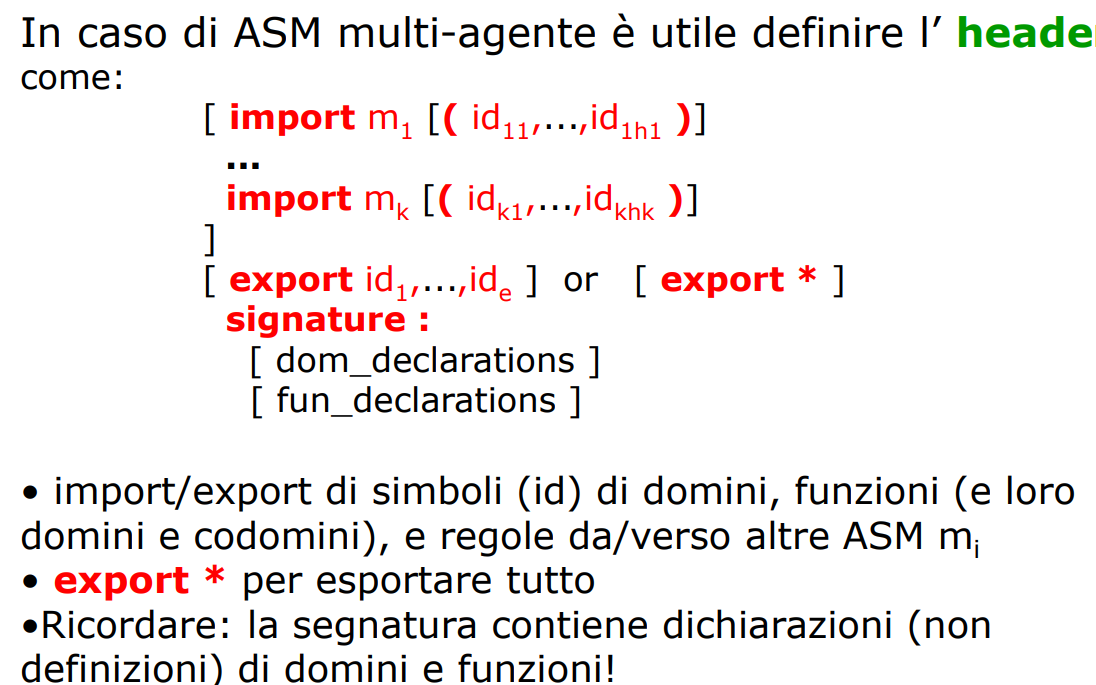
\includegraphics[width=0.8\linewidth]{chapters/3/immaginette/HeaderMultiA.png}
\end{figure}

\subsection{Computazione di ASM multiagenti}
\subsubsection{ASM sincrone: computazione}
\noindent Tutte le ASM lavorano in parallelo:
\begin{itemize}
    \item L'insieme opera negli stati globali, ottenuti dall'unione di tutti gli stati delle ASM componenti
    \item La sequenza di eventi che determina un'esecuzione è la sequenza degli stati che rappresentano l'esecuzione della sync-ASM
\end{itemize}
\noindent una \textbf{multi-agent ASM con agenti sincroni} ha una \textit{quasi-sequential run}
\begin{itemize}
    \item una sequenza di stati $S_0$, $S_1$,… $S_n$,… dove ciascun stato $S_i$ è ottenuto dal precedente $S_{i-1}$ eseguendo in parallelo le regole di tutti gli agenti
\end{itemize}

\subsubsection{ASM asincrone: computazione}
\noindent Nelle async-ASM, gli agenti possono eseguire con clock diversi ed i loro step
possono avere durate diverse
\begin{itemize}
    \item Non c'è il concetto di controllo globale del sistema
    \item Possiamo dare delle \textit{proprietà delle run}
    \item Difficoltà di gestione della consistenza
\end{itemize}

\noindent Una \textit{multi-agent ASM con agenti asincroni} ha una run parzialmente ordinata, ossia un insieme
parzialmente ordinato (M,<) di mosse \textit{m} 
\begin{center}
    leggi: mossa = applicazioni di regole; m1 $<$ m2 se m1 è eseguita prima di m2
\end{center} 
\noindent dei suoi agenti che soddisfano le condizioni:
\begin{itemize}
    \item \textbf{storia finita}: ad un certo istante \textit{t}  la sequenza di mosse che
    ha condotto dallo stato $S_0$ allo stato $S_t$ è finita (ciascuna mossa ha solo un numero finito di
    predecessori)
    \begin{itemize}
        \item per ogni \textit{m} $\in$ \textit{M} l'insieme $\{m' | m' < m\}$ è finito
    \end{itemize}
    \item \textbf{ sequenzialità degli agenti}: ogni agente opera in modo sequenziale
    \begin{itemize}
        \item l'insieme di mosse $\{m | m \in M $, \textit{a} esegue \textit{m}\} di ogni agent \textit{a} $\in$ Agent è linearmente ordinato per $<$
    \end{itemize}
    \item \textbf{ coerenza: ogni stato di M è il risultato delle mosse di agenti}: 
    \begin{itemize}
        \item Sia X un segmento iniziale finito (sottinsieme chiuso a sinistra) di (M,$<$)
        \item Sia $\sigma$(X) lo stato associato ad X: $\sigma$(X) è il risultato di tutte le mosse m in X  
        \item Ciascun segmento iniziale finito X di (M,<) ha uno stato associato $\sigma$(X) che è il risultato dell'applicazione della mossa \textit{m} nello stato $\sigma$(X $-$ \{\textit{m}\}), per ogni elemento massimale \textit{m} $\in$ X 
    \end{itemize}
\end{itemize}
